\chapter{Problèmes d'optimisation sans contrainte à grande échelle}
\label{chap:large-scale}

\section{Introduction}

Les applications pratiques peuvent comporter des centaines ou des milliers de variables.
Avec les techniques des chapitres précédents, nous pouvons être confrontés à des coûts élevés :
\begin{itemize}
    \item Coûts de calcul (temps CPU).
    \item Coûts de stockage (mémoire).
\end{itemize}

Dans ce chapitre, nous présenterons des techniques pour surmonter ces difficultés.

\section{Méthodes de Newton Inexactes}

Dans les méthodes de Newton, on trouve la direction $p_k^N$ en résolvant le système linéaire :
\[
    \nabla^2 f_k p_k^N = - \nabla f_k.
\]
(Formellement, $p_k^N = - (\nabla^2 f_k)^{-1} \nabla f_k$).

\paragraph{Notre objectif} est de trouver une approximation $p_k$ de $p_k^N$ qui n'est pas trop coûteuse à calculer : ce sont les méthodes de Newton inexactes.
Par exemple, nous pouvons utiliser des méthodes itératives comme le gradient conjugué pour résoudre le système de manière approchée.

La qualité de l'approximation déterminera les propriétés de convergence.

\subsection{Convergence locale}

Il est raisonnable d'arrêter la résolution du système $\nabla^2 f_k p_k^N = -\nabla f_k$ lorsque le résidu
\[
    r_k = \nabla^2 f_k p_k + \nabla f_k
\]
est petit.

Par exemple, en utilisant une \textbf{suite forçante} $(\eta_k) \in (0, 1)^\mathbb{N}$ et en arrêtant lorsque :
\begin{equation}
    \| r_k \| \le \eta_k \| \nabla f_k \|.
\end{equation}

Les deux théorèmes de cette sous-section s'appliquent à toutes les méthodes de Newton inexactes satisfaisant la condition ci-dessus.
(Preuves : \textit{Dembo et al.})

\begin{theoreme}[Convergence locale]
    Supposons que $\nabla^2 f(x)$ existe et est continue dans un voisinage d'un minimiseur $x^\star$, avec $\nabla^2 f(x^\star)$ définie positive.
    Soit $x_{k+1} = x_k + p_k$ (où l'on suppose un pas unitaire $\alpha_k=1$ près de la solution) où $p_k$ satisfait :
    \[
        \| r_k \| \le \eta_k \| \nabla f_k \|.
    \]
    Supposons que $\eta_k \le \eta$ pour tout $k$, où $\eta \in [0, 1)$.

    Alors, si $x_0$ est assez proche de $x^\star$, la suite $(x_k)$ converge vers $x^\star$.
    De plus, il existe un certain $\hat{\eta} \in (\eta, 1)$ tel que :
    \[
        \| \nabla^2 f(x^\star) (x_{k+1} - x^\star) \| \le \hat{\eta} \| \nabla^2 f(x^\star) (x_k - x^\star) \|.
    \]
\end{theoreme}

\subsection{Taux de convergence}

\begin{theoreme}[Taux de convergence]
    Supposons les conditions du théorème précédent vérifiées, et que $(x_k)$ converge vers $x^\star$.
    \begin{itemize}
        \item Le taux de convergence est \textbf{super-linéaire} si $\lim_{k \to \infty} \eta_k = 0$.
        \item Si $\nabla^2 f$ est Lipschitz-continue près de $x^\star$ et si $\eta_k = O(\| \nabla f_k \|)$, alors la convergence est \textbf{quadratique}.
    \end{itemize}
\end{theoreme}

\paragraph{Éléments de preuve.}
On peut montrer que :
\[
    \frac{\| \nabla f_{k+1} \|}{\| \nabla f_k \|} \le \eta_k + o(1).
\]
\begin{itemize}
    \item Si $\eta_k \to 0$, alors le gradient (et donc les itérés) converge super-linéairement.
    \item Si $\nabla^2 f$ est Lipschitzienne, on a $\nabla f_{k+1} = O(\| \nabla f_k \|^2)$, ce qui implique une convergence quadratique.
\end{itemize}

\paragraph{Remarques.}
\begin{itemize}
    \item Le choix $\eta_k = \min(0.5, \sqrt{\| \nabla f_k \|})$ donne une convergence \textbf{super-linéaire}.
    \item Le choix $\eta_k = \min(0.5, \| \nabla f_k \|)$ donne une convergence \textbf{quadratique}.
    \item Ces résultats sont locaux : nous avons supposé que $x_0$ était proche de $x^\star$ et que $\alpha_k = 1$.
\end{itemize}

\subsection{Méthodes Newton-CG avec recherche linéaire}

On résout le système $\nabla^2 f_k p_k = - \nabla f_k$ en utilisant la méthode du gradient conjugué (CG).
Nous devons arrêter si nous rencontrons une direction de courbure négative (c'est-à-dire si $\nabla^2 f_k$ n'est pas définie positive).

\section{Méthodes Quasi-Newton à mémoire limitée (L-BFGS)}

Lorsque la Hessienne n'est pas disponible à un coût raisonnable (en temps ou en stockage), les méthodes Quasi-Newton à mémoire limitée sont utiles.
Elles remplacent le stockage de matrices $n \times n$ par le stockage d'un nombre limité de vecteurs de taille $n$.
Nous nous concentrons ici sur la méthode \textbf{L-BFGS} (Low-storage BFGS), qui stocke l'information sur la courbure des $m$ itérations précédentes.
(Dérivation : \textit{\cite{nocedal1980updating}}).

\subsection{Rappels sur BFGS}

Les étapes de BFGS sont $x_{k+1} = x_k - \alpha_k H_k \nabla f_k$, où $H_k$ est mis à jour selon :
\begin{equation}
    H_{k+1} = V_k^\top H_k V_k + \rho_k s_k s_k^\top,
\end{equation}
avec $V_k = I - \rho_k y_k s_k^\top$ et $\rho_k = \frac{1}{y_k^\top s_k}$.
On note $s_k = x_{k+1} - x_k$ et $y_k = \nabla f_{k+1} - \nabla f_k$.

\subsection{Principes de L-BFGS}

\begin{itemize}
    \item Au lieu de stocker la matrice dense $H_k$, nous stockons $m$ paires de vecteurs $(s_i, y_i)$.
    \item À chaque itération, nous substituons la paire la plus ancienne $(s_{k-m}, y_{k-m})$ par la nouvelle $(s_k, y_k)$.
    \item En pratique, on choisit $m$ entre 3 et 20.
    \item À l'itération $k$, nous disposons de l'itéré courant $x_k$ et des paires $(s_i, y_i)$ pour $i = k-m, \dots, k-1$.
    \item On choisit une approximation initiale $H_k^0$.
\end{itemize}

\begin{figure}[htbp]
\centering
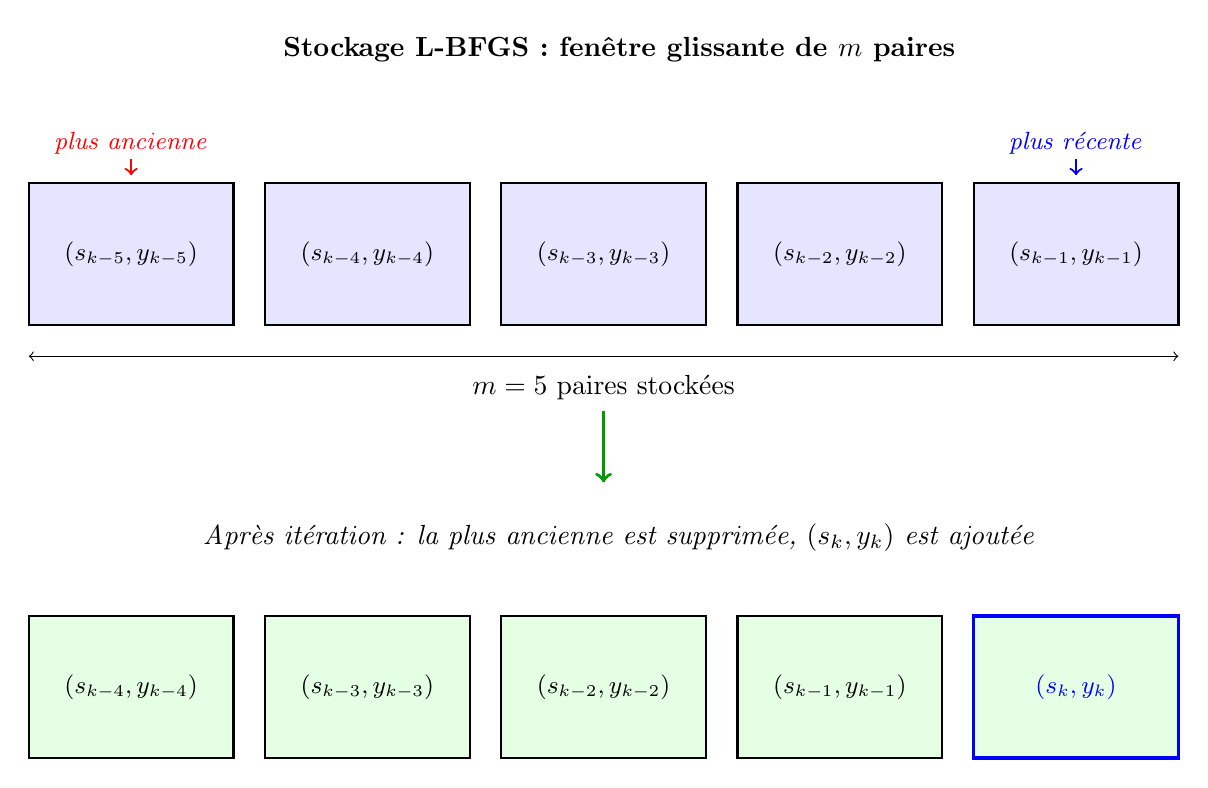
\begin{tikzpicture}[scale=1.0]
    % Title
    \node at (7.5, 3.5) {\textbf{Stockage L-BFGS : fenêtre glissante de $m$ paires}};
    
    % Memory slots (boxes) - wider spacing
    \foreach \i in {0,...,4} {
        \draw[thick, fill=blue!10] (\i*3, 0) rectangle (\i*3+2.6, 1.8);
    }
    
    % Labels for stored pairs - use smaller subscripts
    \node[font=\small] at (1.3, 0.9) {$(s_{k-5}, y_{k-5})$};
    \node[font=\small] at (4.3, 0.9) {$(s_{k-4}, y_{k-4})$};
    \node[font=\small] at (7.3, 0.9) {$(s_{k-3}, y_{k-3})$};
    \node[font=\small] at (10.3, 0.9) {$(s_{k-2}, y_{k-2})$};
    \node[font=\small] at (13.3, 0.9) {$(s_{k-1}, y_{k-1})$};
    
    % Oldest label
    \node[red, font=\small] at (1.3, 2.3) {\textit{plus ancienne}};
    \draw[->, red, thick] (1.3, 2.1) -- (1.3, 1.9);
    
    % Newest label  
    \node[blue, font=\small] at (13.3, 2.3) {\textit{plus récente}};
    \draw[->, blue, thick] (13.3, 2.1) -- (13.3, 1.9);
    
    % m label at bottom
    \draw[<->] (0, -0.4) -- (14.6, -0.4);
    \node at (7.3, -0.8) {$m = 5$ paires stockées};
    
    % Vertical arrow between states - positioned after label
    \draw[->, very thick, green!60!black] (7.3, -1.1) -- (7.3, -2.0);
    
    % New state after update - more vertical space
    \begin{scope}[shift={(0, -5.5)}]
        \node at (7.5, 2.8) {\textit{Après itération : la plus ancienne est supprimée, $(s_k, y_k)$ est ajoutée}};
        
        \foreach \i in {0,...,4} {
            \draw[thick, fill=green!10] (\i*3, 0) rectangle (\i*3+2.6, 1.8);
        }
        
        \node[font=\small] at (1.3, 0.9) {$(s_{k-4}, y_{k-4})$};
        \node[font=\small] at (4.3, 0.9) {$(s_{k-3}, y_{k-3})$};
        \node[font=\small] at (7.3, 0.9) {$(s_{k-2}, y_{k-2})$};
        \node[font=\small] at (10.3, 0.9) {$(s_{k-1}, y_{k-1})$};
        \node[blue, font=\small\bfseries] at (13.3, 0.9) {$(s_k, y_k)$};
        
        % New pair highlight
        \draw[blue, very thick] (12, 0) rectangle (14.6, 1.8);
    \end{scope}
\end{tikzpicture}
\caption{Principe du stockage L-BFGS : fenêtre glissante de $m$ paires $(s_i, y_i)$. À chaque itération, la paire la plus ancienne est éliminée et la nouvelle paire est ajoutée.}
\label{fig:lbfgs-storage}
\end{figure}

\begin{figureexplanation}
La figure~\ref{fig:lbfgs-storage} illustre le principe de stockage de L-BFGS. Au lieu de maintenir la matrice $H_k$ (de taille $n \times n$), on conserve uniquement les $m$ dernières paires de vecteurs $(s_i, y_i)$. Cette approche réduit le coût de stockage de $O(n^2)$ à $O(mn)$, ce qui est essentiel pour les problèmes de grande dimension.
\end{figureexplanation}

On peut développer la formule de mise à jour de manière récursive :
\begin{align*}
    H_k &= V_{k-1}^\top H_{k-1} V_{k-1} + \rho_{k-1} s_{k-1} s_{k-1}^\top \\
    &= V_{k-1}^\top (V_{k-2}^\top H_{k-2} V_{k-2} + \rho_{k-2} s_{k-2} s_{k-2}^\top) V_{k-1} + \rho_{k-1} s_{k-1} s_{k-1}^\top \\
    &= \dots \\
    &= (V_{k-1}^\top \dots V_{k-m}^\top) H_k^0 (V_{k-m} \dots V_{k-1}) \\
    &\quad + \rho_{k-m} (V_{k-1}^\top \dots V_{k-m+1}^\top) s_{k-m} s_{k-m}^\top (V_{k-m+1} \dots V_{k-1}) \\
    &\quad + \dots + \rho_{k-1} s_{k-1} s_{k-1}^\top.
\end{align*}

Cette formule permet de calculer le produit $H_k \nabla f_k$ sans jamais former la matrice $H_k$ (voir Algorithme~\ref{alg:lbfgs-twoloop}, \textit{two-loop recursion}).

\paragraph{Complexité.}
L'Algorithme~\ref{alg:lbfgs-twoloop} requiert $4mn$ opérations, plus le coût du calcul de $H_k^0 q$ ($n$ multiplications si $H_k^0$ est diagonale).

\paragraph{Choix de $H_k^0$.}
En pratique, choisir $H_k^0 = \gamma_k I$ avec :
\begin{equation}
    \gamma_k = \frac{s_{k-1}^\top y_{k-1}}{y_{k-1}^\top y_{k-1}},
\end{equation}
donne des résultats satisfaisants. On peut montrer que $\gamma_k$ approche une des valeurs propres de la Hessienne.

\paragraph{Recherche linéaire.}
Comme pour BFGS, on utilise les conditions de Wolfe (fortes) et on initialise la recherche linéaire avec $\alpha_k = 1$.
